\chapter{Dipolo elettrico}

Due \mkeyword{dipolo elettrico} cariche puntiformi $+ q$ e $-q$ mantenute a una distanza fissa $a$ costituiscono un dipolo elettrico. \\
\mkeyword{momento del dipolo}Si chiama momento del dipolo elettrico il vettore 

\begin{equation}
    \mathbf{p} = q  \mathbf{a}
\end{equation}

Dove $\mathbf{a}$ è orientato dalla carica negativa a quella positiva.

\begin{figure}[h]
    \centering
    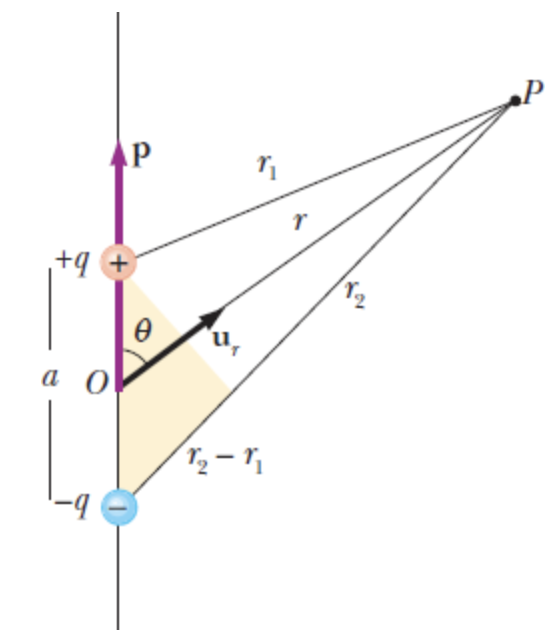
\includegraphics[width=0.4\linewidth]{figure/image12.png}
    \caption{Dipolo elettrico}
    \label{fig:chapter_6_1}
\end{figure}

Il potenziale elettrostatico del dipolo si trova con la \ref{eq:potenziale_per_più_cariche}:

\begin{equation*}
    V(P) = \frac{q}{4 \pi \varepsilon_0} (\frac{1}{r_1} - \frac{1}{r_2}) = \frac{q}{4 \pi \varepsilon_0}  \frac{r_2 - r_1}{r_1 r_2}
\end{equation*}

Se il punto $P$ è molto lontano dal dipolo, cioè $r \gg a $ (condizione detta approssimazione di dipolo), si può porre

\begin{equation}
    r_2 - r_1 = a \cos \theta \quad , \quad r_1 r_2 = r^2
\end{equation}

E quindi 

\begin{tcolorbox}[colback=yellow!10!white, colframe=orange!70!black, boxrule=0.8pt]
\begin{equation}
    V(P) = \frac{p \cos \theta}{4 \pi \varepsilon_0 r^2} = \frac{\mathbf{p} \cdot \mathbf{u}_r}{4 \pi \varepsilon_0 r^2}
    \label{eq:potenziale_dipolo}
\end{equation}
\end{tcolorbox}

Dalla formula si nota che l'unica grandezza caratteristica del dipolo è il momento $\mathbf{p}$ e non $q$ e $a$ separatamente: questo significa che da \emph{misure di potenziale elettrostatico possiamo ricavare informazioni du $\mathbf{p}$ ma non sulla costituzione del sistema}. \\
Geometricamente è spontanea la scelta delle coordinate polari sferiche aventi polo $O$ nel centro del dipolo. 

Andiamo a calcolare il campo elettrostatico con la \ref{eq:Campoelettrostatico_come_gradiente}:

\begin{align}
    E_r = - \frac{\partial V}{\partial r} = \frac{2 p \cos \theta}{4\pi \varepsilon_0 r^3}, \\ E_{\theta} =- \frac{1}{r} \frac{\partial V}{\partial \theta} = \frac{p \sin \theta}{4 \pi \varepsilon_0 r^3}\\
    E_{\varphi} = 0 \qquad \quad
\end{align}

Vettorialmente 

\begin{tcolorbox}[colback=yellow!10!white, colframe=orange!70!black, boxrule=0.8pt]
\begin{equation}
    \mathbf{E} = E_r \mathbf{u}_r + E_{\theta} \mathbf{u}_{\theta} = \frac{p}{4 \pi \varepsilon_0 r^3} (2 \cos \theta \ \mathbf{u}_r + \sin \theta \ \mathbf{u}_{\theta})
    \label{eq:componenti_campo_dipolo}
\end{equation}
\end{tcolorbox}

E il modulo vale 

\begin{equation}
    E = \frac{p}{4 \pi \varepsilon_0} \sqrt{3 \cos^2 \theta + 1}
\end{equation}

Tuttavia se si esprime il momento di dipolo in componenti polari:

\begin{equation}
    \mathbf{p} = p \cos \theta \ \mathbf{u}_r - p \sin \theta \ \mathbf{u}_{\theta} \implies p \sin \theta \ \mathbf{u}_{\theta} = p \cos \theta \ \mathbf{u}_r - \mathbf{p}
\end{equation}

Sostituendo nella \ref{eq:campo_dipolo} si ottiene 

\begin{tcolorbox}[colback=yellow!10!white, colframe=orange!70!black, boxrule=0.8pt]
\begin{equation}
    \mathbf{E} = \frac{1}{4 \pi \varepsilon_0 r^3} (3p \cos \theta \ \mathbf{u}_r - \mathbf{p}) = \frac{1}{4 \pi \varepsilon_0 r^3} \left [ 3(\mathbf{p} \cdot \mathbf{u}_r) \ \mathbf{u}_r - \mathbf{p}\right ]
\label{eq:campo_dipolo}
\end{equation}
\end{tcolorbox}

In particolare il secondo termine nel secondo membro rappresenta la componente antiparallela a $\mathbf{p}$.

\begin{figure}[h]
    \centering
    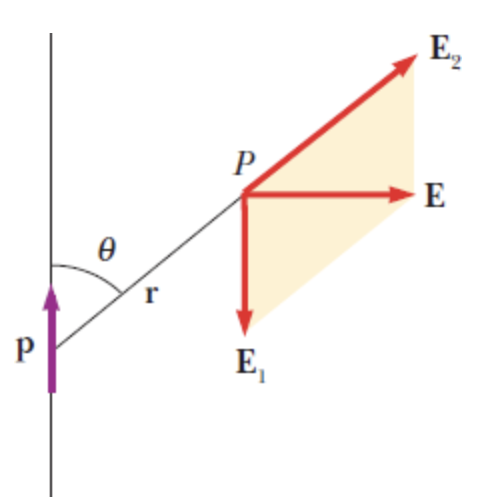
\includegraphics[width=0.4\linewidth]{figure/image13.png}
    \caption{Rappresentazione del un campo elettrostatico di un dipolo elettrico}
    \label{fig:campo_dipolo}
\end{figure}

\newpage

\section{Potenziale di una distribuzione di cariche nell'approssimazione di dipolo}

L'espressione \ref{eq:potenziale_dipolo} dedotta per il potenziale di due cariche puntiformi eguali e opposte può essere generalizzata per sistemi di cariche più complessi. \\

Consideriamo un sistema di cariche $q_i$ distribuite in una regione ristretta di dimesione massima $d$.

\begin{figure}[h]
    \centering
    \begin{subfigure}{0.48\textwidth}
        \centering
        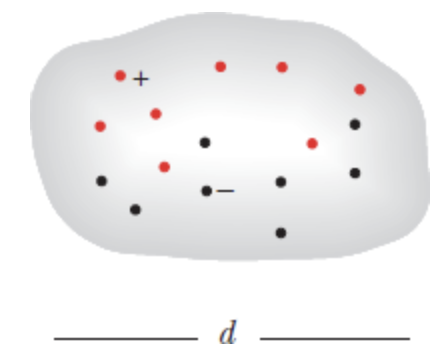
\includegraphics[width=0.7\linewidth]{figure/image14.png}
        \caption{Distribuzione di cariche }
        \label{fig:sub1}
    \end{subfigure}
    \hfill
    \begin{subfigure}{0.48\textwidth}
        \centering
        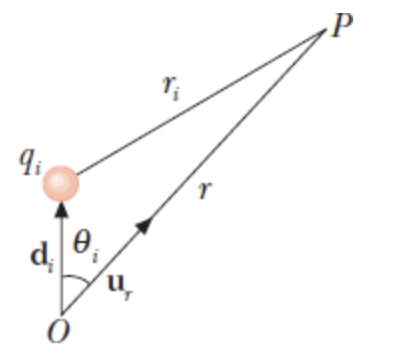
\includegraphics[width=0.7\linewidth]{figure/image15.png}
        \caption{Approssimazione di dipolo}
        \label{fig:sub2}
    \end{subfigure}
    %\caption{Confronto tra due campi elettrici}
    \label{fig:campi}
\end{figure}


Detto $O$ un qualsiasi punto interno alla regione, calcoliamo il potenziale elettrostatico in un punto $P$ a distanza $r$ da $O$ molto grande rispetto a $d \quad (r \gg d)$. Se $r_i$ è la distanza da $q_i$ a $P$

\begin{equation*}
    V = \frac{1}{4 \pi \varepsilon_0} \sum _i \frac{q_i}{r_i}
\end{equation*}

Chimando $\mathbf{d}_i$ il vettore che unisce $O$ alla carica $q_i$, abbiamo $\mathbf{d}_i + \mathbf{r}_i = \mathbf{r}$ e se vale $r \gg d_i$ possiamo scrivere

\begin{equation}
    r_i \approx r - d_i \cos \theta_i = r - \mathbf{d}_i \cdot \mathbf{u}_r
\end{equation}

Con $\mathbf{u}_r$ versore della direzione $OP$. Pertanto

\begin{equation}
    \frac{1}{r_i} \approx \frac{1}{r -\mathbf{d}_i \cdot \mathbf{u}_r} = \frac{r + \mathbf{d}_i \cdot \mathbf{u}_r}{r^2 - (\mathbf{d}_i \cdot \mathbf{u}_r)^2} \approx \frac{r + \mathbf{d}_i \cdot \mathbf{u}_r}{r^2 }
\end{equation}

Sostituendo nel potenziale 

\begin{equation}
    V \approx \frac{1}{4 \pi \varepsilon_0} \frac{\sum_i q_i (r + \mathbf{d}_i \cdot \mathbf{u}_r)}{r^2} =\frac{Q}{4 \pi \varepsilon_0 r} + \frac{(\sum_i q_i \mathbf{d}_i ) \cdot \mathbf{u}_r}{4 \pi \varepsilon_0 r^2}
\end{equation}

Definiamo il vettore \mkeyword{monento di dipolo di un sistema }

\begin{equation}
    \mathbf{p} = \sum_i q_i \ \mathbf{d} _i
\end{equation}

detto momento di dipolo elettrico del sistema rispetto al punto $O$ e quindi vale 

\begin{tcolorbox}[colback=yellow!10!white, colframe=orange!70!black, boxrule=0.8pt]
\begin{equation}
    V \approx \frac{Q}{4 \pi \varepsilon_0 r} + \frac{\mathbf{p} \cdot \mathbf{u}_r}{4 \pi \varepsilon_0 r^2} = V_0 + V_{\text{dip}}
\end{equation}
\end{tcolorbox}

\newpage

Il primo termine \mkeyword{monopolo} rappresenta il potenziale elettrostatico generato da una carica, eguale alla carica totale del sistema, posta nel punto $O$ e si chiama termine monopolo. Il secondo, formalmente uguale a \ref{eq:potenziale_dipolo}, si chiama termine di dipolo. \mkeyword{dipolo}\\

Se la $Q$ è diversa da zero il termine di monopolo è preponderante, infatti scrivendo 

\begin{equation*}
    \mathbf{p} = \sum_i q_i \mathbf{d}_i \approx Q \ \mathbf{d}
\end{equation*}

dove il modulo di $\mathbf{d}$ non è molto diverso dai moduli dei vari $\mathbf{d}_i$, abbiamo

\begin{equation*}
    \frac{V_{\text{dip}}}{V_0} = \frac{\mathbf{p} \cdot \mathbf{u}_r}{r Q} \approx \frac{Q d}{r Q} = \frac{d}{r} \ll 1
\end{equation*}

Se invece il sistema è neutro $(Q = 0)$, il termine di monopolo è nullo e il potenziale in $P$ è \emph{dato solo dal termine di dipolo}.\\

\' E possibile andare a schematizzare un sistema neutro pensandolo come due cariche $+ Q$ e $-Q$ poste a una certa distanza. \\

Per un sistema di $n$ cariche di un segno e $n$ cariche eguali ma di segno opposto possiamo scrivere

\begin{equation}
    \mathbf{p} = \sum_i q_i \mathbf{d}_i ^{(+)} - \sum_i q_i \mathbf{d}_i ^{(-)} = Q \ \mathbf{d}_1 - Q \ \mathbf{d}_2
\end{equation}

Quindi l'esistenza di un momento di dipolo in una distribuzione di cariche è legata all'esistenza di un' \emph{asimmetria}.\\

Quando $\mathbf{p} = 0$ il dipolo \mkeyword{termini di multipolo} non è sufficiente per il calcolo del potenziale, occorre introdurre nuovi termini che prendono il nome di termini di multipolo. 

\newpage

\section{Forza su un dipolo elettrico}

Consideriamo un dipolo elettrico avente centro in $O \equiv (x,y,z)$  e formato da una carica $-q$ posta in $P_1 \equiv (x - \frac{a_x}{2}, y - \frac{a_y}{2}, z - \frac{a_z}{2} )$ e in $P_2 \equiv (x + \frac{a_x}{2}, y + \frac{a_y}{2}, z + \frac{a_z}{2} )$; il vettore $\mathbf{a} = a_x \mathbf{u}_x + a_y \mathbf{u}_y + a_z \mathbf{u}_z$ congiunge $P_1$ e $P_2$ e il momento di dipolo è $\mathbf{p} = q \ \mathbf{a}$. 

\begin{figure}[h]
    \centering
    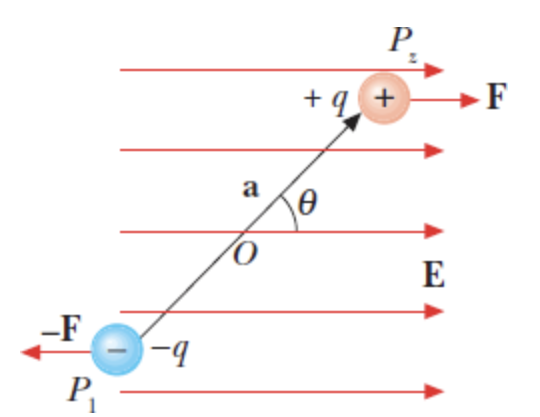
\includegraphics[width=0.4\linewidth]{figure/image16.png}
    \caption{Dipolo elettrico in un campo elettrostatico}
    \label{fig:dipolo_campo_elettrostatico}
\end{figure}

Se il dipolo si trova in un campo elettrostatic $\mathbf{E}$, la sua energia potenziale risulta essere

\begin{equation*}
U_e = q V(P_2) - q V(P_1) = q  [V(P_2) - V(P_1)]
\end{equation*}

Se la distanza $a$ è piccola (cosa che accade spesso nei dipoli), possiamo andare ad applicare il teorema del differenziale totale e scrivere

\begin{tcolorbox}[colback=yellow!10!white, colframe=orange!70!black, boxrule=0.8pt]
\begin{equation}
    U_e \approx q \ a_x \ \frac{\partial V}{\partial x} + q \ a_y \ \frac{\partial V}{\partial y}  + q \ a_z \ \frac{\partial V}{\partial z}  = \mathbf{p} \cdot \nabla V = - \mathbf{p \cdot \mathbf{E}} = - p \cos \theta \ E
    \label{eq:energia_potenziale_dipolo}
\end{equation}
\end{tcolorbox}

Dove \emph{le derivate parziali sono calcolate nel centro del dipolo}

\subsection{Campo elettrostatico uniforme}

Supponiamo che il campo elettrostatico in cui è immerso il dipolo sia uniforme, allora le forze sulle cariche $\mathbf{F}_1 = - q \ \mathbf{E}$, $\mathbf{F}_2 = q \ \mathbf{E}$, costituiscono una \emph{coppia} e quindi hanno risultante nulla.\\

Tuttavia il \emph{momento meccanico è diverso da zero}. Facendo ruotare il dipolo di un angolo $\theta$ rispetto alla posizione di equilibrio stabile, il dipolo risente di un momento delle forze $\mathbf{M}$ rispetto al centro del dipolo

\begin{equation}
    \mathbf{M} = \mathbf{r}_1 \times \mathbf{F}_1 + \mathbf{r}_2 \times \mathbf{F}_2 = (\mathbf{r}_2 - \mathbf{r}_1) \times q \ \mathbf{E} = q \ \mathbf{a} \times \mathbf{E} = \mathbf{p} \times \mathbf{E}
\end{equation}

Quindi vale 

\begin{tcolorbox}[colback=yellow!10!white, colframe=orange!70!black, boxrule=0.8pt]
\begin{equation}
    \mathbf{M} =\mathbf{p} \times \mathbf{E} =  - p \sin \theta \  E \  \mathbf{u}_z = - \frac{\partial U_e}{\partial \theta} \mathbf{u}_z
\end{equation}
\end{tcolorbox}

\subsection{Campo elettrostatico non uniforme}

Supponiamo, adesso, che il dipolo sia immerso in un campo elettrostatico non uniforme, in questo caso, oltre al momento $\mathbf{M}$, agisce una forza risultante $\mathbf{F}$, poiché le forze sulle due cairche $-q$ e $+q$ sono ora diverse in quanto diverso è il valore del campo elettrostatico nelle due posizioni. 

\begin{equation*}
    \mathbf{F}_1 = -q \ \mathbf{E}_1 \quad , \quad \mathbf{F}_2 = q \ \mathbf{E}_2 = q (\mathbf{E}_ + \frac{\partial \mathbf{E}}{\partial x} a_x  + \frac{\partial \mathbf{E}}{\partial y} a_y  + \frac{\partial \mathbf{E}}{\partial z} a_z )
\end{equation*}

Dove abbiamo sfruttato il teorema del differenziale totale. 

\begin{figure} [h]
    \centering
    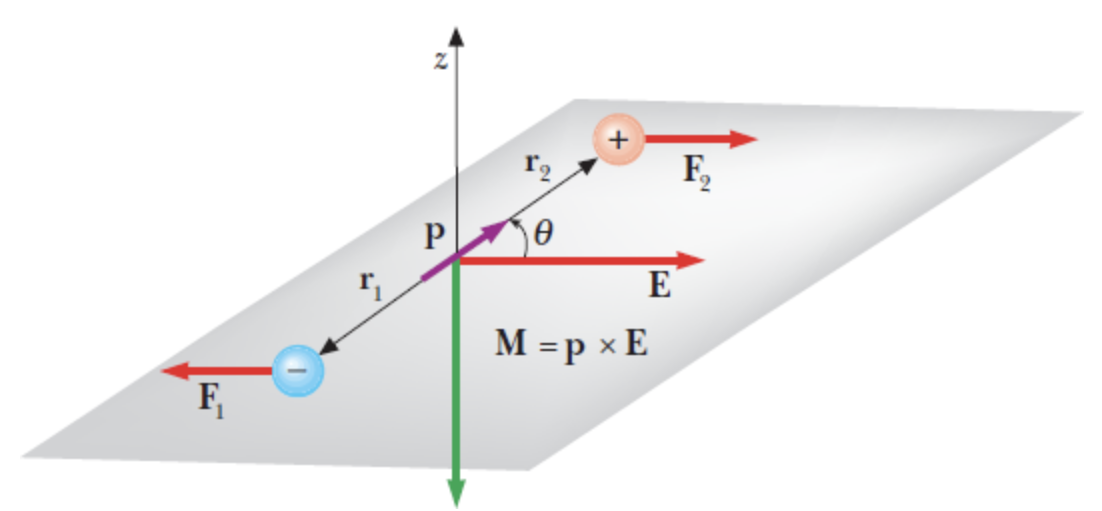
\includegraphics[width=0.6\linewidth]{figure/image17.png}
    \caption{Dipolo in un campo elettrostatico non uniforme}
    \label{fig:dipolo_campo_non_uniforme}
\end{figure}

La forza risultante è 

\begin{equation*}
    \mathbf{F} = \mathbf{F}_1 + \mathbf{F}_2 = q \ \mathbf{E}_2 = q \ a_x   \frac{\partial \mathbf{E}}{\partial x} + q \ a_y \frac{\partial \mathbf{E}}{\partial y}  + q \ a_z \frac{\partial \mathbf{E}}{\partial z}  
\end{equation*}

Ovvero 

\begin{tcolorbox}[colback=yellow!10!white, colframe=orange!70!black, boxrule=0.8pt]
\begin{equation}
    F = p_x \frac{\partial \mathbf{E}}{\partial x} + p_y \frac{\partial \mathbf{E}}{\partial y} + p_z \frac{\partial \mathbf{E}}{\partial z} = (\mathbf{p} \cdot \nabla) \ \mathbf{E}
\end{equation}
\end{tcolorbox}

\subsection{interazione tra dipoli}

Due dipoli elettrici di momenti elettrici $\mathbf{p}_1$ e $\mathbf{p}_2$, posti a distanza $r$ tra di loro, interagiscono in quanto ciascuno è sottoposto al campo elettrostatico dell'altro. 

\begin{figure}[h]
    \centering
    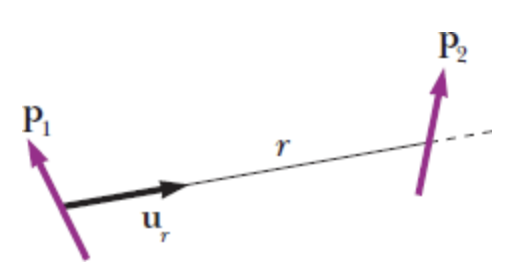
\includegraphics[width=0.4\linewidth]{figure/image18.png}
    \caption{Interazione tra dipoli}
    \label{fig:interazione_dipoli}
\end{figure}

Riprendendo la \ref{eq:potenziale_dipolo} e la \ref{eq:campo_dipolo}, si ottiene che il potenziale del secondo dipolo è 

\begin{equation}
    U_{e,2} = - \mathbf{p}_2 \cdot \mathbf{E}_1 = \frac{1}{4 \pi \varepsilon_0 r^3} [\mathbf{p}_1 \cdot \mathbf{p_2} - 3(\mathbf{p}_1 \cdot \mathbf{u}_r)(\mathbf{p}_2 \cdot \mathbf{u}_r) ]
\end{equation}

\newpage

Dove $\mathbf{u}_r$ è il versore della direnzione che va dal primo al secondo dipolo. Si vede che l'energia potenziale è simmetrica rispetto allo scambio di 1 e 2, quindi $U_{e,1} = U_{e,2}$. \\

La forza subita dal secondo dipolo è 

\begin{equation}
    \mathbf{F}_2 = - \nabla U_e 
\end{equation}

Si nota che la componente $r$ (supponendo di essere in coordinate sferiche) della forza è proporzionale a $1/r^4$

\begin{equation*}
    F_r  \propto \frac{1}{r^4}
\end{equation*}

quindi l'interazione decresce molto velocemente con la distanza.
